\chapter{Stacks for the multiple myeloma microenvironment}
\label{Chap:Stacks}

\section{Introduction}

The tumor microenvironment is an incredibly important component in the development and progression of cancer \cite{Hanahan2012, Whiteside2008, Lorusso2008}. 3D \invitro\ models are commonly used to investigate components and mechanisms within the human tumor microenvironment as they have been shown to better recapitulate many \invivo\ phenomena \cite{Sung2013, Fischbach2007, Hickman2014Three-dimensionalVivo., stock2016capturing, Baker2012, Debnath2005, Wu2014, Asghar2015}. The models can be as simple as cells seeded in scaffolds, or complex layers of cells and matrix 3D printed to create structure. An important feature that these \invitro\ tumor models enable is study how the microenvironement can enhance tumorogesis and how cancer changes the microenvironment to promote tumor progression \cite{Verbridge2010, Chandler2012, Ingber2008, Polyak2009}. There are ample methods to investigate how tumors interact with their microenvironment, however, as models become more complex to achieve better biological relevance, it becomes more difficult to isolate individual signals and their sources. We have developed a modular tumor microevnrionment platform that is capable dynamic assembly and disassembly of its components. 

There have been several examples of using modular assembly methods for developing tissue. Modular culture methods were developed to be able to avoid issues with larger tissue scaffolds such as uneven oxygen and nutrient penetration into an \invitro\ tissue. Once, mature these smaller tissues are assembled into perfusion systems to allow growth into larger tissues for tissue engineering applications. Modular tissue constructs were not designed to be disassembled and were largely seen as a tool to make larger tissue constructs, not necessarily as a research tool for investigating interactions within the tissue \cite{Lovett2009, Lee2012a, Bruzewicz2008, Nichol2009}.

We are using this platform to investigate the multiple myeloma (MM) tumor microenvironment. MM is an incredibly complex disease that is defined by the interactions that occur within the tumor microenvironment \cite{Mahindra2010a, Manier2012, Ribatti2006}. Understanding the signals and interactions that occur within the MM microenvironment will give us a better understanding of how the disease progresses, especially under stresses of therapy, and lead to potential improvments in how the disease is managed and treated.

\section{Methods}

\subsection{Fabrication}
Stacks and device holders devices were designed in 3D CAD software. Prototype devices were CNC milled from 1.2 mm thick crystalline polystyrene sheets. Devices used for tissue culture were redesigned to have pinning features on both top and bottom of the device and injection molded. The injection molded devices were sprayed treated with a layer of SEBS dissolved in limonene to enhance the hydrophobic properties of the surface. Treated devices were sonicated in isopropyl alcohol overnight to remove limonene from the SEBS coating. The devices were stored in ethanol until used for experiments. Stacks device holders were 3D printed from food-grade poly(lactic acid) using fused deposition modeling. 

\subsection{Multiple myeloma bone marrow culture}
We created a bone marrow scaffold with a mixture of ECM components previously used in the literature and optimized for viability and structural stability for this application \cite{Reagan2014, DiBuduo2015, Torisawa2014, Wenger2004, Morrison2014}. The ECM mixture was seeded with 750 cells/\textmu L (either HS-5 BMSCs or a mixture of MSCs and HS-5s) for a final concentration of: 2.5 mg/mL growth factor reduced Matrigel, 1 mg/mL rat tail collagen I, 0.5 mg/mL sodium hyaluronate, and 7.5 mg/mL fibrinogen diluted into RPMI media with 10\% FBS, 2\% GlutaMax, 1\% Pen Strep, and 12.5 mM HEPES. 4 \textmu L of cell-laded scaffold was pipetted into each well of the stacks device then placed in the tissue culture incubator for between 2 and 4 hours for the scaffold to gel. Devices were removed from the incubator and 10 \textmu L of warm RPMI media was added to the top of each well. The devices were then returned to the incubator and left for 2 days. 

After 2 days, MM cell line, MM.1S were added to the culture. New devices were loaded with MM.1S cells 4 \textmu L at 1500 cells/\textmu\ in RPMI media. The two stacks devices were assembled with the bone-marrow stack placed on top of the MM stack allowing for soluble factor signalling to occur without cell crossover. The devices were returned to the incubator and media was changed daily by aspirating the 10 \textmu L droplet sitting on each well and replacing it with fresh media. 

\subsection{Bortezomib dose response}
After 5 days of coculture the bone marrow and MM stacks layers were separated. MM cells in suspension culture were collected and centrifuged. The media supernatant from coculture was aspirated and cells were resuspended at 100 cells/\textmu L of fresh RPMI media. Cells that were to be treated with borezomib on the 1st day of monoculture were seeded at 10 \textmu L each into a 384 well plate, and the remainder of the culture was seeded into a 24-well plate at 500 \textmu per well. Bortezomib was added to MM cells in the 384 well plate at concentrations from 0 to 100 nM. The following day cells treated with bortezomib were stained with a live/dead kit, imaged, and analyzed for number of cells viable or dead at each concentration. Cells treated with bortezomib at days 2 and 6 were collected from the 24-well plate and transfered to the 384-well plate in the same manner as described. Viability as a function of bortezomib concentration for each day was fit to a 4-parameter sigmoid curve and IC50 values were determined. 


\section{Results and discussion}

\subsection{Stacks design}

The stacks were designed to be a modular multiculture platform where cultures could be prepared separately, joined together and exchange fluid both the top and bottom, then removed. The modularity in this system enabled a time-based approach to tissue culture that is fairly difficult to achieve even with a Transwell. The wells in stacks are designed to be open on the top and bottom of the device allowing arrangement in multiple orientations and making the assembly of two or more separate cultures relatively simple \ref{figure:StacksFig1}A).

The most pressing design need in this system is to contain fluid to where it needs to be. This is an open microculture system that can be completely disassembled with no tubing, no channels, and no bonding so fluid containment is not trivial. The device was designed so that fluid could be added and removed from the wells and not leak at the interface between wells. This was achieved through both material choice by making the surface more hydrophobic with SEBS to discourage wetting of surfaces and the geometry is designed to pin water at the interface. At the interface the space between to the layers is very small, the small gap is a feature that encourages fluid wetting through spontaneous capillary flow (SCF). To prevent leaking across the entire surface of the device, a gap feature was integrated into the design at each well. This gap is sharp (at a 90\degree angle) and the gap is large enough to prevent SCF. The result is a stable interface where fluid is pinned when the device is assembled, and can then be taken apart and reassembled without compromising the interface (Figure \ref{figure:StacksFig1}B).

\begin{figure}[h!] %DONE
\centering
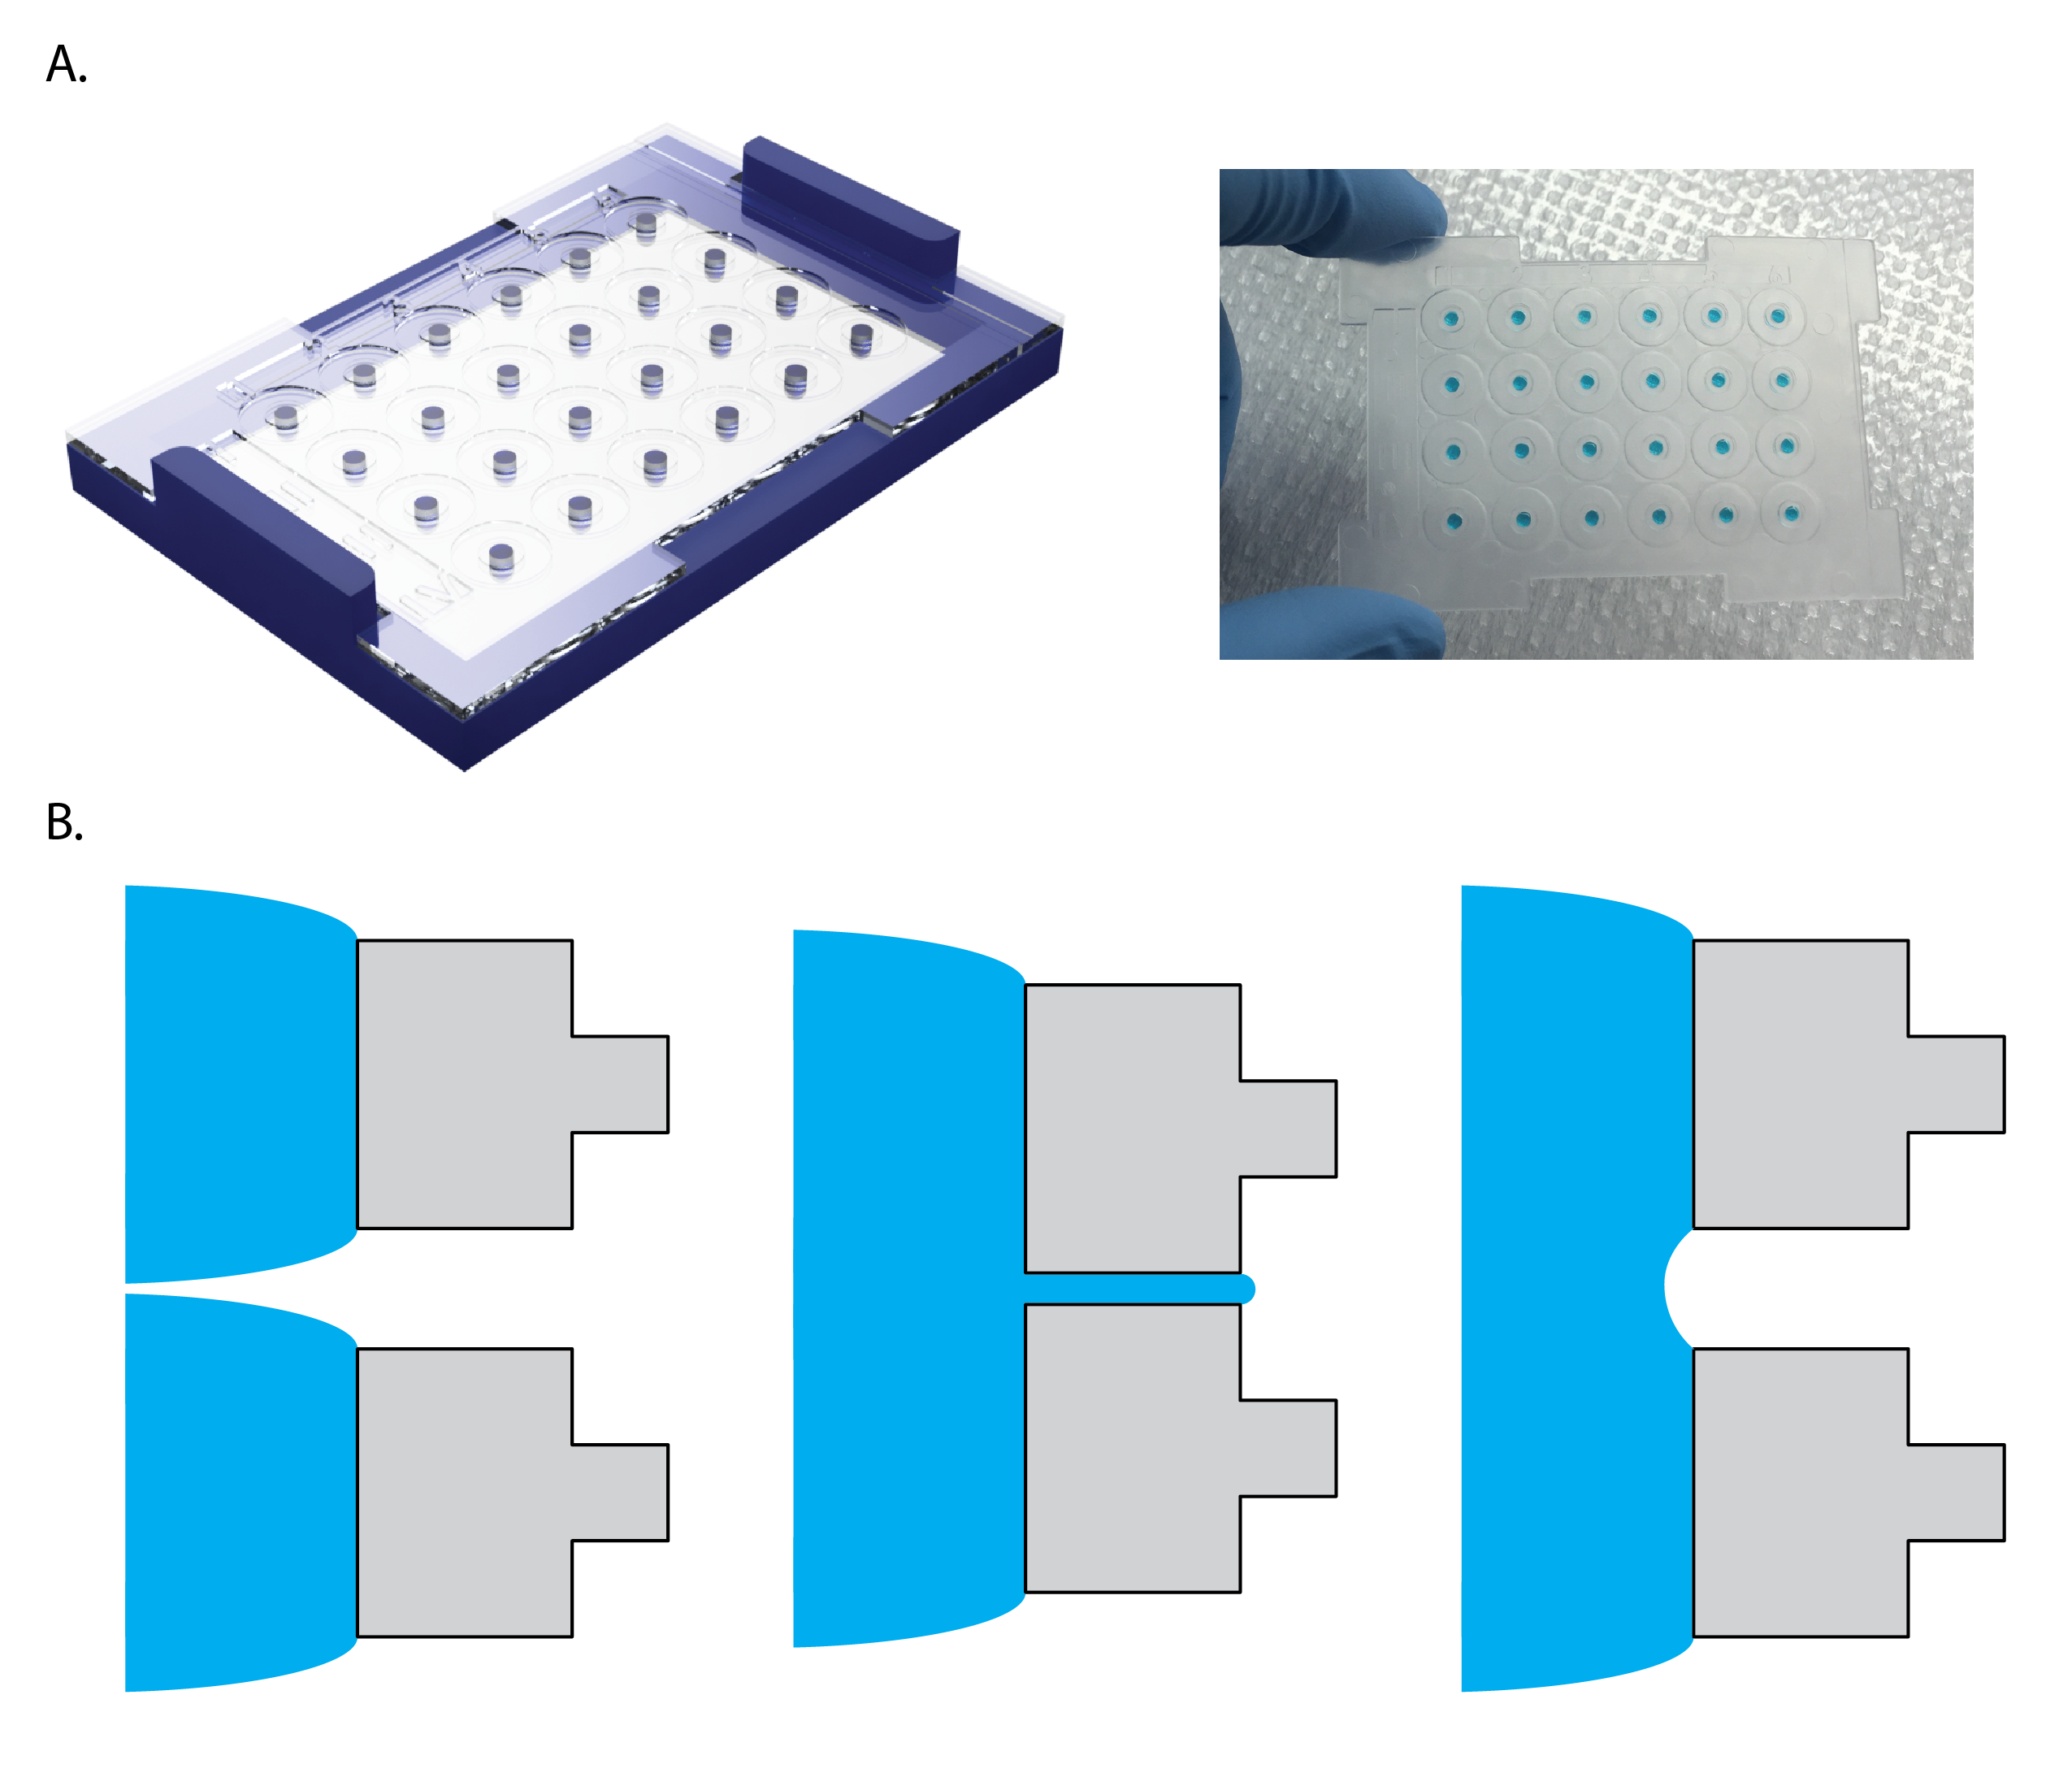
\includegraphics[width=5.75in]{/StacksFig1.png}
\caption[\textbf{Stacks device and operation}]{\textbf{Stacks device and operation.} (A) 3D rendering and photograph of device loaded with fluid. (B) Device assembly and disassembly}
\label{figure:StacksFig1}
\end{figure}


Fluid exchange with the device can be achieved in two ways. The first way is accomplished by changing the fluid droplet that forms on either the top or bottom of the device when more fluid is added than what the well can hold. The second method of fluid exchange is performed with an additional stacks layer. The layer can be filled and place on top of a stacks device or stacks assembly allowing. When fluid needs to be exchanged the exchange layer is removed, fluid is aspirated, and new fluid can be added and returned to the assembly.

Interestingly, is the fact that fluid exchange in the stacks platform is achieved removing fluid from a droplet that has formed on top of the device and not the bottom. This is unintuitive since it has previously been observed in a open well device that fluid added that exceeds the capacity of the well tends to form a droplet underneath the device in response to gravity \cite{DeGroot2016}. Even more curious this phenomena was only observed in the injection molded device and not in the micromilled prototype, where media pooled underneath the device. We believe this can be explained due to the specific feature of drafting that was incorporated into the design of the injection molded device to allow for easier release from the mold. The drafting of the injection molded creates a well that is wider on top than on bottom. This difference in radii creates a difference in pressures between the two droplets with the larger radii droplet having a lower pressure than the smaller radii droplet. 
When fluid is initially added to the well, the difference is pressure is able to overcome gravity creating two differently sized droplets. As more fluid is added the pressure in the top droplet continues getting larger and relative pressure continues to get lower overcoming gravity. To test this hypothesis, the device was operated upside down (smaller radius on top) and fluid formed a droplet on the bottom face of the device (Figure \ref{figure:StacksFig2}A. The feature of the device that allows for fluid to be exchanged from the top and not the bottom enables the hanging droplet culture of MM cells without disruption of the system without an additional fluid exchange layer greatly simplifying media replenishment and treatment additions. The device has a height of 1.2 mm, but a simplified version of the Young-Laplace equations assuming spherical droplets at equilibrium (Equation \ref{equation:StacksEq1}) leads to a maximum device height of approximately 1.8 mm given the same radii in this particular device to maintain top-side pooling, a steeper draft angle would enable taller devices. 

\begin{equation}
    \frac{1}{r_{b}} = \frac{1}{r_{t}}+ \frac{\rho gh}{2\gamma}
    \label{equation:StacksEq1}
\end{equation}

We have tested droplet formation experimentally in devices experimentally by operating the device with the drafting facing upwards (Figure \ref{figure:StacksFig2}B), and downwards (Figure \ref{figure:StacksFig2}C). We observed large droplets of fluid forming on top of the device when the larger radius was facing upwards, and the opposite effect when the larger side was facing downards.

\begin{figure}[h!] %DONE
\centering
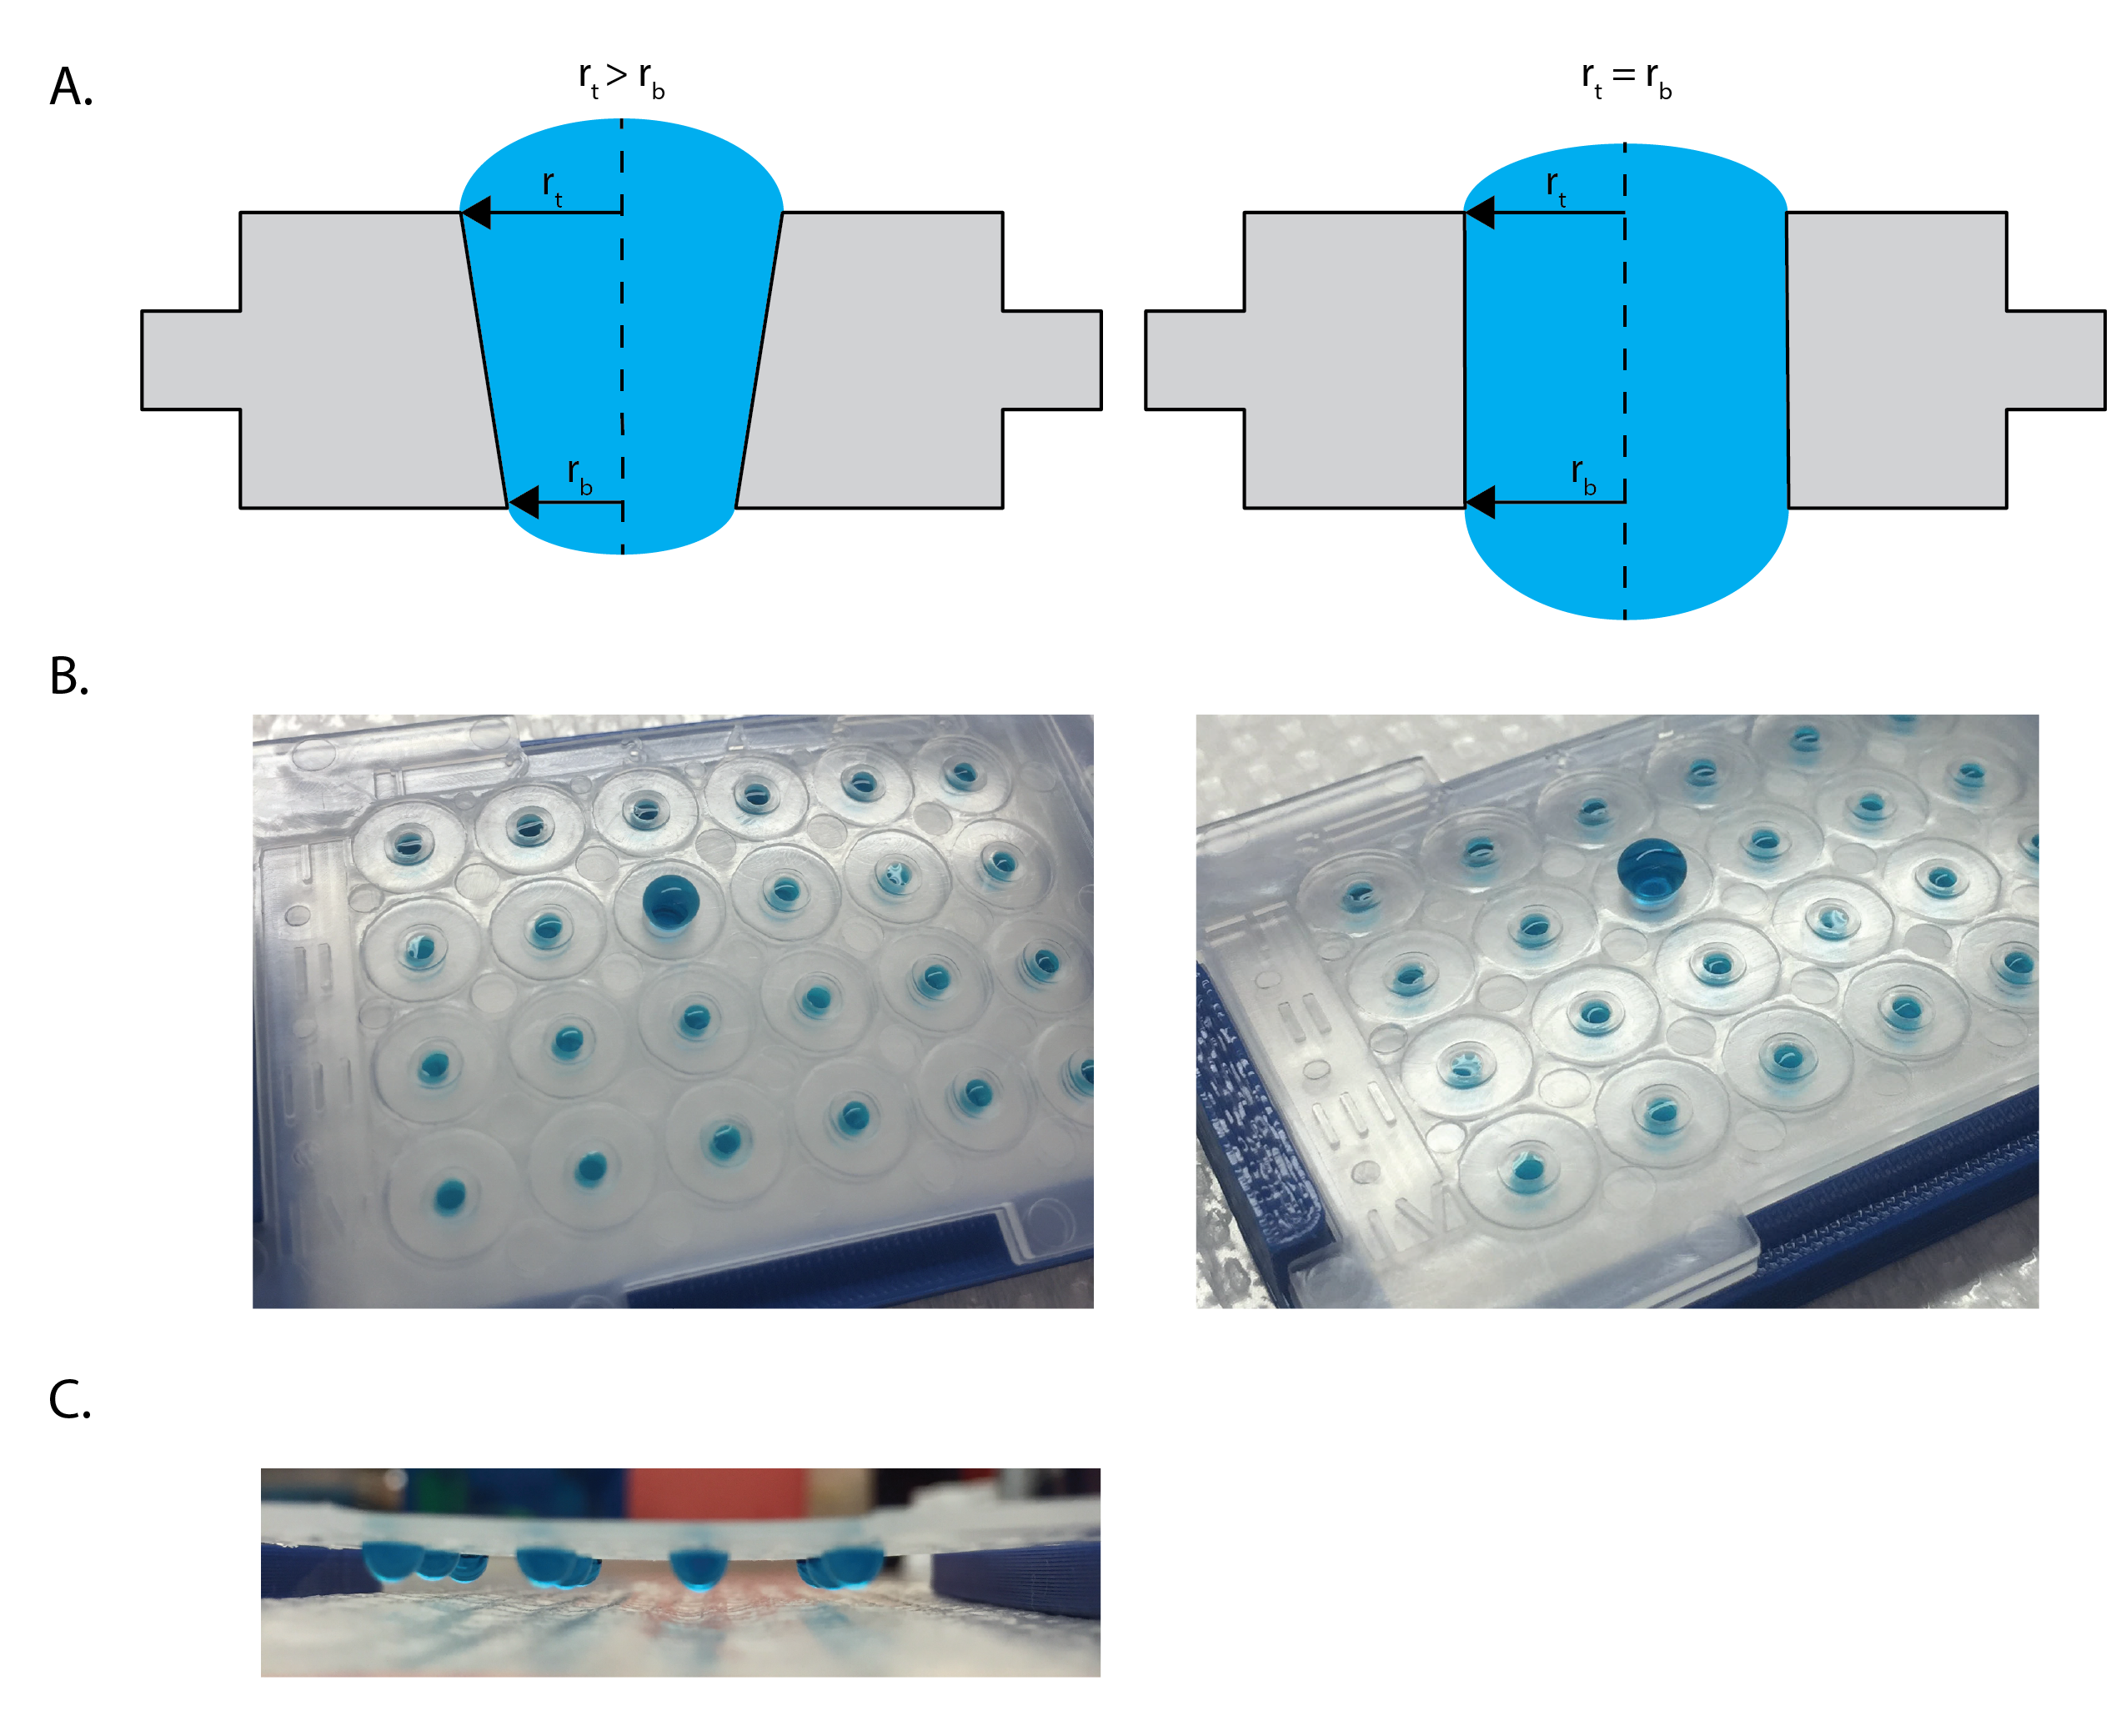
\includegraphics[width=5.75in]{/StacksFig2.png}
\caption[\textbf{The effect of slope on droplet formation}]{\textbf{The effect of slope on droplet formation.} (A) Illustration of drafted device (left) and straight device (right) and how fluid pools in each once it has exceeded the volume of the well. (B) Image of fluid added to device when larger radius side is facing upwards at 15 \textmu L (left) and 30 \textmu L (right). (C) Image of fluid (30 \textmu L) pooling underneath device when operated with the larger radius side of the device facing downward.}
\label{figure:StacksFig2}
\end{figure}

\subsection{MM Model}
We were able to leverage the modularity of the stacks platform to develop a two part multiple myeloma microenvironment model. The model consists of both, a solid bone marrow microenvironmental model and a liquid MM model. Each of the models were prepared separately in the stacks device then joined together to enable soluble factor signalling, though physically separate (Figure \ref{figure:StacksFig3}A). Since the cells are not intermixed, they are able to be entirely separated following culture, then recombined as desired. We have leveraged this capability to investigate the effects of coculture on drug response of MM cells. It has been shown that coculture of bone marrow stromal cells can provide a protective effect against drug treatments targeting MM cells \cite{Abdi2013}, using stacks we are not only able to study how these effects can change in a 3D biomimetic based on soluble cues, but also investigate how persistent the protective signals are over time once two-way communication has stopped. We have investigated how MM cells behave in response to bortezomib treatment following periods of coculture with BMSCs. We compared coculture response to bortezomib of the MM.1S cell line with bone marrow cells derived from both healthy individuals and individuals diagnosed with MM. Falling in line with our expectations, BMSCs derived from MM patients provided additional protection against bortezomib-induced cell death (Figure \ref{figure:StacksFig3}A). We then studied how MM cells respond to bortezomib as a function of time in monoculture, following a period of coculture (Figure \ref{figure:StacksFig3}. Immediate treatment with bortezomib of MM cells following removal of BMSC signals resulted in a fairly high IC50 value. 48 hours following separation from coculture, the MM cells became dramatically more sensitive to bortezomib and has a similar IC50 value to 6 days of monoculture. This time course experiment demonstrates that some signals that are present in coculture are maintained for brief times, and resistance to bortezomib requires consituitive signalling to be maintained, in this system at least. 

\begin{figure}[h!] %DONE
\centering
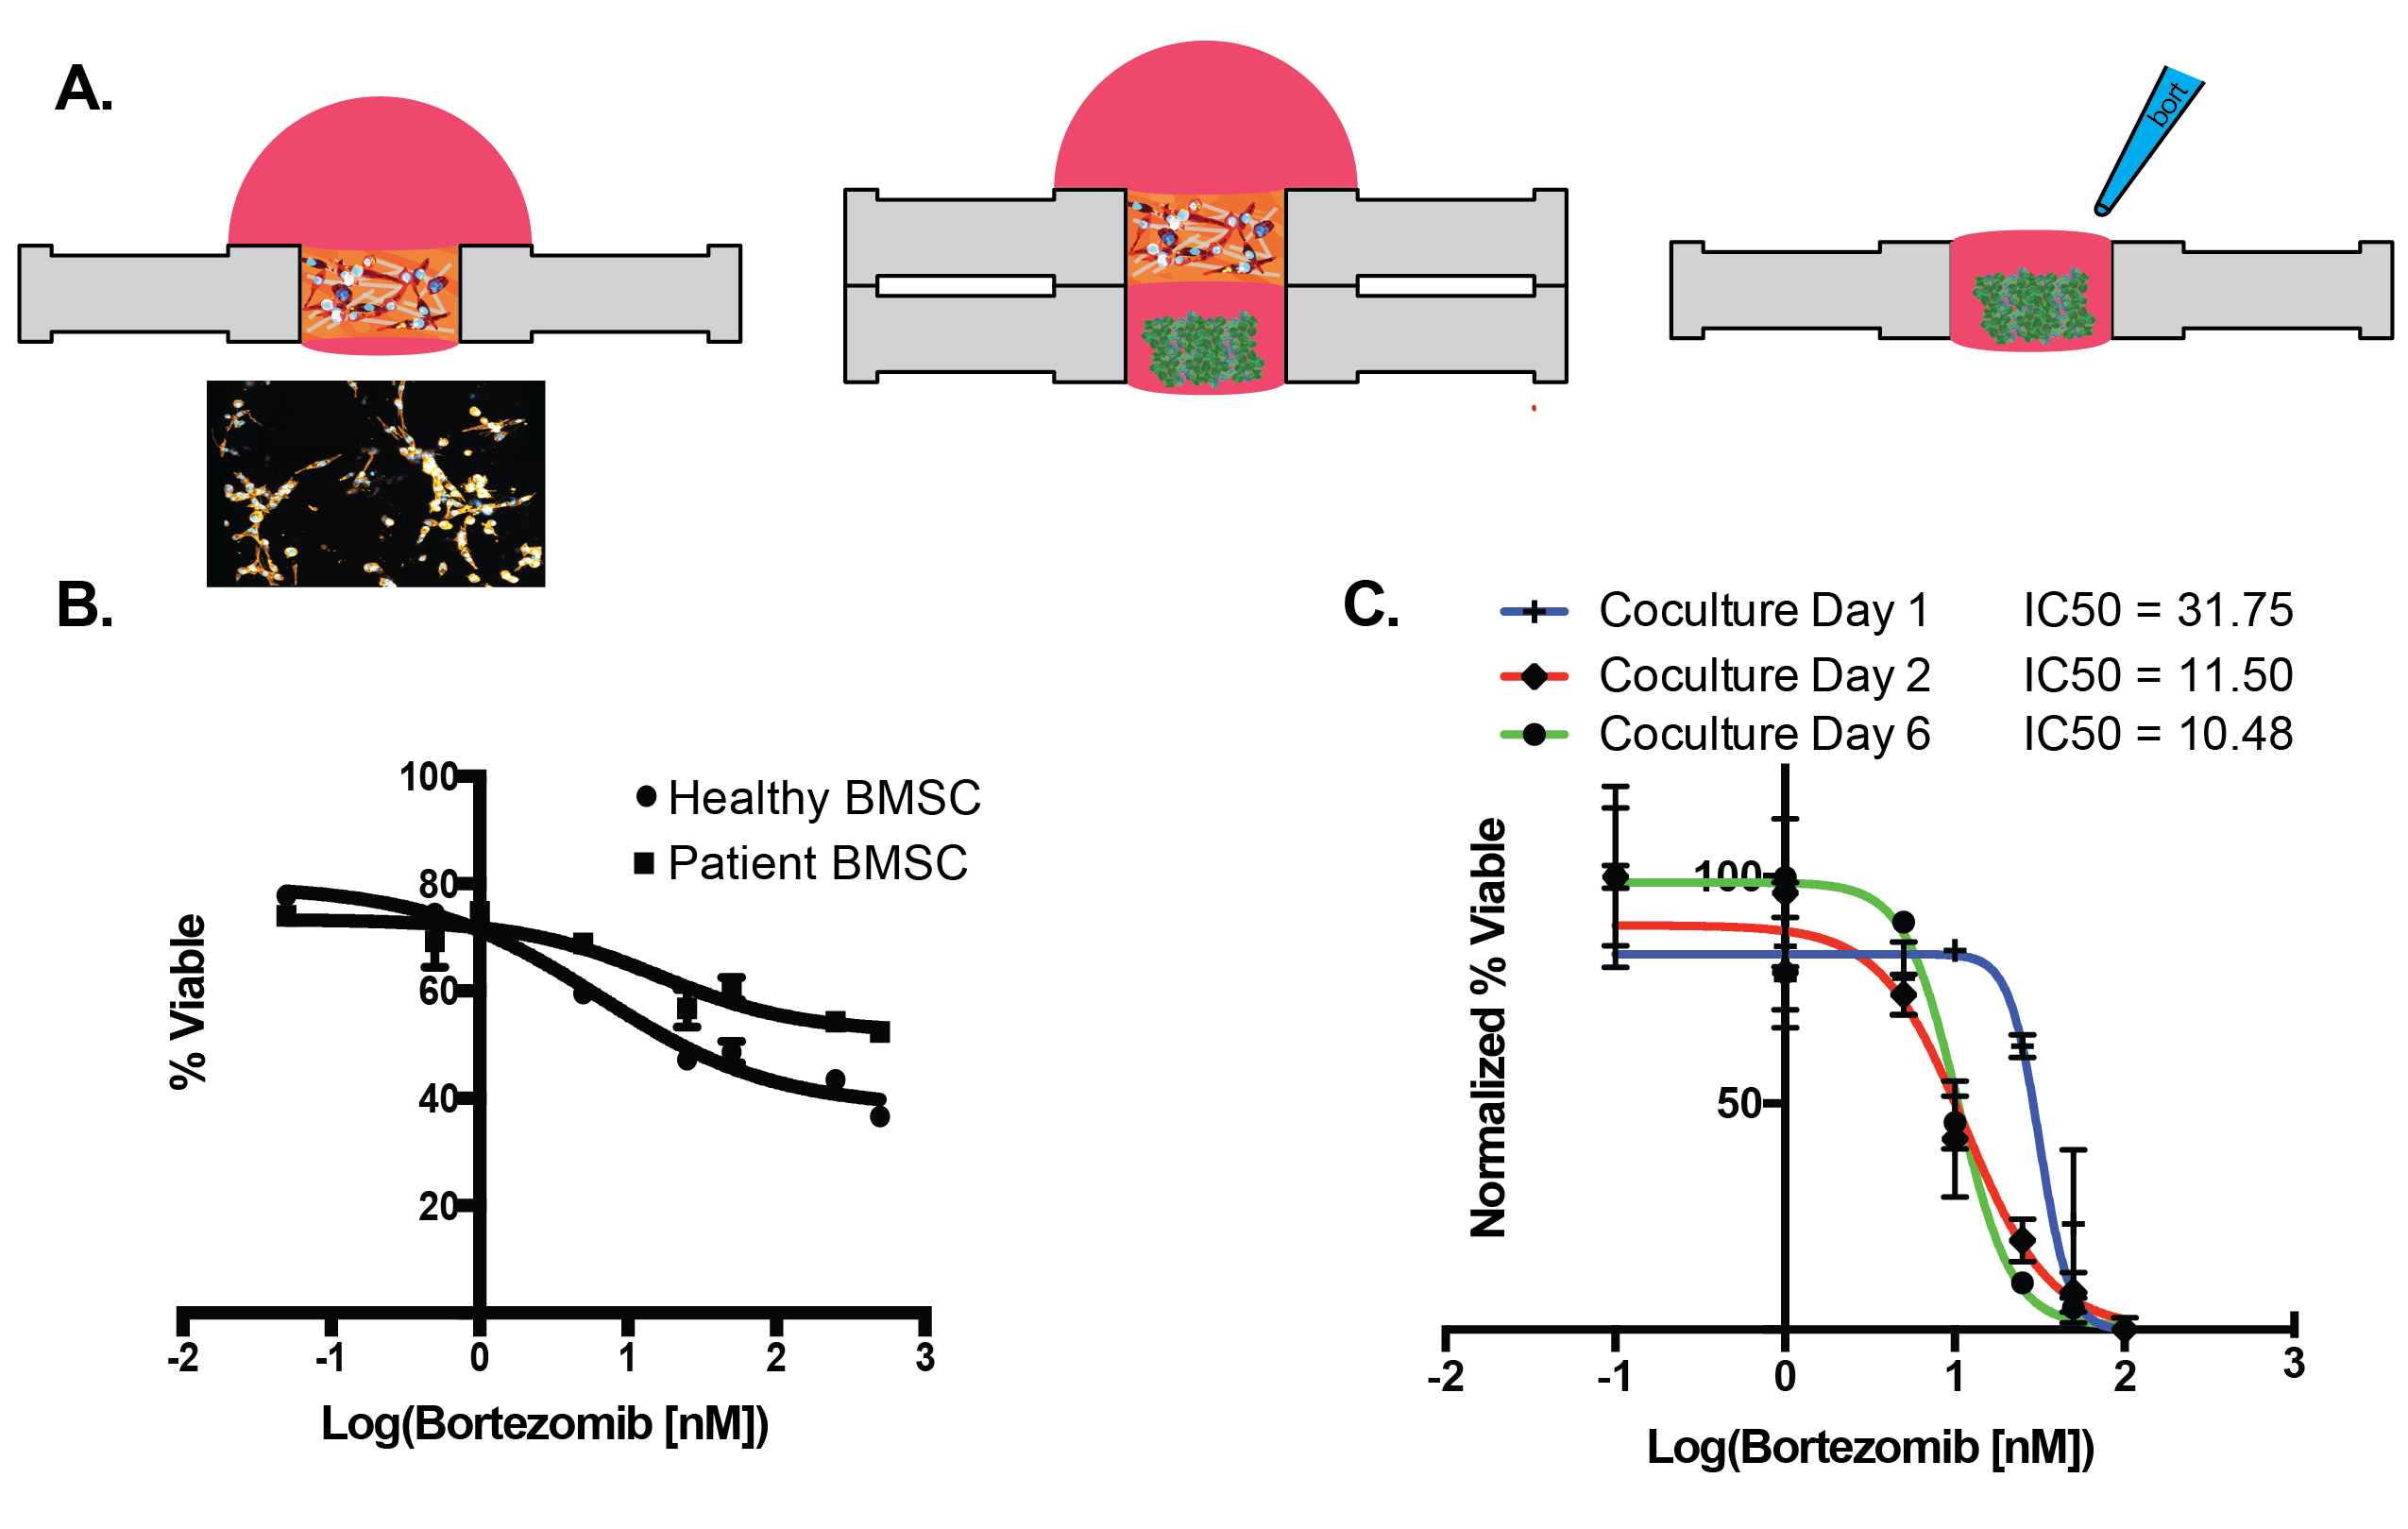
\includegraphics[width=5.75in]{/StacksFig3.png}
\caption[\textbf{Stacks for MM microenvironment coculture}]{\textbf{Stacks for MM microenvironment coculture.} (A) Illustration of experimental time line from left to right. BMSCs are seeded into a bone marrow-like sacffold in a stacks layer. The BMSC layer is joined with a layer containing a liquid culture of MM cells. After a period of coculture the two layers are separated and the MM layer is treated with bortezomib. (B) Dose response curve to bortezomib of MM cells cocultured with healthy BMSCs and patient BMSCs. (C) Dose response curve to bortezomib over time of MM cells cocultured with BMSCs in after being placed in monoculture.}
\label{figure:StacksFig3}
\end{figure}

\section{Conclusion}
We were able to develop well-based microfluidic system that is fairly simple to use but allows for advanced control over culture scenarios. We have shown this platform to be not only amenable for high throughput fabrication \textit{via} injeciton molding, but that injection molding actually improved the features of the device by making easier to operate and enable not only solid, but also liquid culture. We demonstrated some preliminary success in developing a model for the MM microenvironment, but further development is required to fully exploit the modularity of the system to enable new biology to be studied. 